\documentclass{article}

\usepackage[left=2cm,right=2cm,top=2cm,bottom=2cm]{geometry} 

\usepackage[utf8]{inputenc}   % otra alternativa para los caracteres acentuados y la "ñ"
\usepackage[           spanish % para poder usar el español
                      ,es-tabla % para los captions de las tablas
                       ]{babel}   
\decimalpoint %para usar el punto decimal en vez de coma para los números con decimales

%\usepackage{beton}
%\usepackage[T1]{fontenc}

\usepackage{parskip}
\usepackage{xcolor}

\usepackage{caption}

\usepackage{fancyvrb}

\usepackage{enumerate} % paquete para poder personalizar fácilmente la apariencia de las listas enumerativas

\usepackage{graphicx} % figuras
\usepackage{subfigure} % subfiguras

\usepackage{amsfonts}
\usepackage{amsmath}

\usepackage[formats]{listings}
\lstdefineformat{R}{~=\( \sim \)}
\lstset{basicstyle=\ttfamily,format=R}

\definecolor{gris}{RGB}{220,220,220}
	
\usepackage{float} % para controlar la situación de los entornos flotantes

\restylefloat{figure}
\restylefloat{table} 
\setlength{\parindent}{0mm}


\usepackage[bookmarks=true,
            bookmarksnumbered=false, % true means bookmarks in 
                                     % left window are numbered
            bookmarksopen=false,     % true means only level 1
                                     % are displayed.
            colorlinks=true,
            allcolors=blue,
            urlcolor=blue]{hyperref}
\definecolor{webblue}{rgb}{0, 0, 0.5}  % less intense blue


\title{\Huge SWAP: Balanceo de carga en un sitio web\vspace{10mm}}

\author{\huge David Cabezas Berrido \vspace{10mm} \\ 
  \huge dxabezas@correo.ugr.es \vspace{10mm}}

\begin{document}
\maketitle
\tableofcontents
\newpage

\section{Preparativos}

Creamos dos archivos \texttt{/var/www/html/index.html} básicos en las máquinas 1 y 2, donde se referencie el número de la máquina a la que
pertenece el archivo para saber cuál de las dos máquinas atendió la petición.

Creamos una nueva máquina virtual M3 con Ubuntu Server, pero no instalamos los servicios de la práctica 1, ya que no podemos
tener a Apache ocupando el puerto 80. Nos limitamos a configurar el doble
adaptador de red como hicimos en las otras dos máquinas. Su dirección IP es 192.168.56.103, para hacer peticiones desde la
máquina anfitriona.

A partir de aquí, todas las órdenes y configuraciones se realizan en M3 a menos que digamos
lo contrario.

\section{Balanceo de carga con NGINX}

Comenzamos instalando y lanzando NGINX:

\begin{verbatim}
	sudo apt-get update && sudo apt-get dist-upgrade && sudo apt-get autoremove
	sudo apt-get install nginx
	sudo systemctl start nginx
\end{verbatim}

Comprobamos que el servicio está en funcionamiento.

\begin{figure}[H]
	\centering
	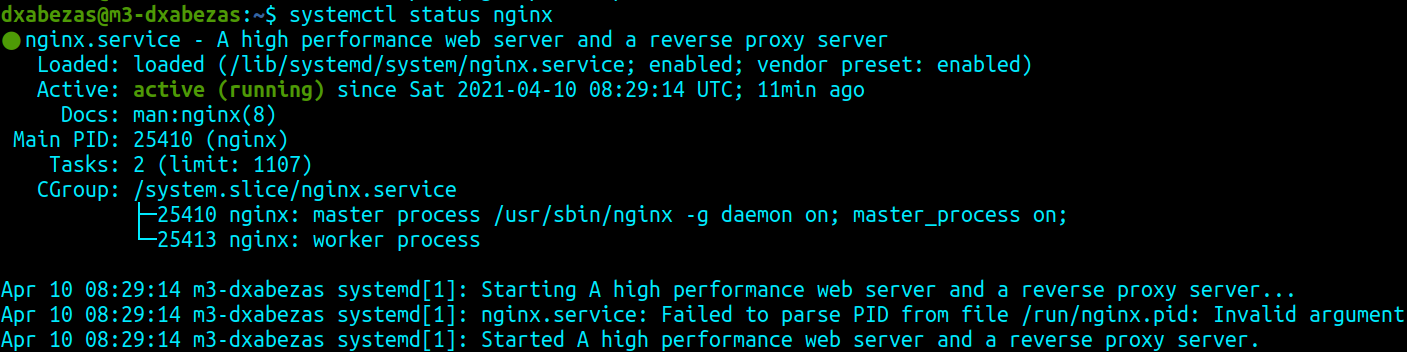
\includegraphics[width=148mm]{imgs/nginx-status}
	\caption{NGINX está activo.}
	\label{fig:nginx-status}
\end{figure}

Escribimos en \texttt{/etc/nginx/conf.d/default.conf} la configuración que se indica en el guión
para que NGINX funcione como balanceador de carga en lugar de como servidor web.

\begin{Verbatim}[tabsize=4]
upstream balanceo_dxabezas {
	server 192.168.56.101;
	server 192.168.56.102;
}

server{
	listen 80;
	server_name balanceador_dxabezas;
	access_log /var/log/nginx/balanceador_dxabezas.access.log;
	error_log /var/log/nginx/balanceador_dxabezas.error.log;
	root /var/www/;

	location /
	{
		proxy_pass http://balanceo_dxabezas;
		proxy_set_header Host $host;
		proxy_set_header X-Real-IP $remote_addr;
		proxy_set_header X-Forwarded-For $proxy_add_x_forwarded_for;
		proxy_http_version 1.1;
		proxy_set_header Connection "";
	}
}
\end{Verbatim}

Reestauramos el servicio con \verb^sudo service nginx restart^, haremos esto (aunque no lo digamos) cada vez que
modifiquemos este fichero. Ahora si visitamos la IP de M3
en el navegador de la máquina anfitriona, observamos que NGINX sigue funcionando como servidor
web.

\begin{figure}[H]
	\centering
	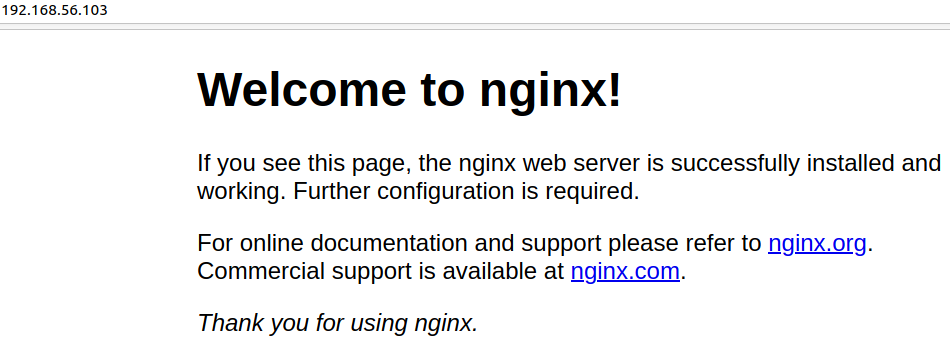
\includegraphics[width=100mm]{imgs/nginx-web}
	\caption{NGINX está funcionando como servidor web.}
	\label{fig:nginx-web}
\end{figure}

Como se nos indica en el guión, comentamos la línea \verb^/etc/nginx/sites-enabled/*;^
del fichero \texttt{/etc/nginx/nginx.conf}. Ahora accedemos a la IP de la máquina 3, y cada vez que refrestamos la página
se turnan las máquinas 1 y 2 para servirnos su \texttt{index.html}.

\begin{figure}[H]
	\centering
	\subfigure{
\includegraphics[width=120mm]{imgs/index-m1}}
	\subfigure{
\includegraphics[width=120mm]{imgs/index-m2}}
	\label{fig:index}
\end{figure}

Ahora añadimos el parámetro \texttt{weight} en el fichero \texttt{/etc/nginx/conf.d/default.conf} para que la máquina 2 reciba
el doble de peticiones que la 1.

\begin{Verbatim}[tabsize=4]
upstream balanceo_dxabezas {
	server 192.168.56.101 weight=1;
	server 192.168.56.102 weight=2;
}
\end{Verbatim}
Si ahora vamos refrescando la página, la máquina que nos atiende en cada momento es: \\
M1, M2, M2, M1, M2, M2, M1, M2, M2, \ldots

Seguidamente, probamos a cambiar el algoritmo de Round-Robin (por defecto) a IP-HASH para que siempre nos atienda la misma máquina,
lo conseguimos añadiendo la directiva \texttt{ip\_hash} en el fichero de configuración.
\begin{Verbatim}[tabsize=4]
upstream balanceo_dxabezas {
	ip_hash;
	server 192.168.56.101;
	server 192.168.56.102;
}
\end{Verbatim}
Ahora, por más que refresquemos la página, nos atiende siempre la misma máquina, en nuestro caso la 2. 

Finalmente, activamos las conexiones con keepalive the 3 segundos.
\begin{Verbatim}[tabsize=4]
upstream balanceo_dxabezas {
	server 192.168.56.101;
	server 192.168.56.102;
	keepalive 3;
}
\end{Verbatim}
Aunque no es sencillo comprobar que funciona correctamente, ya que recargar la página abre una conexión nueva.

Probamos algunas opciones avanzadas más. De las propuestas en el guión, elegiremos aquellas cuyo
funcionamiento podamos comprobar más fácilmente.

\begin{Verbatim}[tabsize=4]
upstream balanceo_dxabezas {
	ip_hash;
	server 192.168.56.101;
	server 192.168.56.102 down;
}
\end{Verbatim}
Marcando M2 como \texttt{down} con \texttt{ip\_hash}, comprobamos que ahora nos atiende M1 en lugar de M2.

\begin{Verbatim}[tabsize=4]
upstream balanceo_dxabezas {
	server 192.168.56.101;
	server 192.168.56.102 backup;
}
\end{Verbatim}
Ahora marcamos M2 como backup y siempre nos atiende M1. Si desactivamos el servicio de M1 con \\
\verb^sudo systemctl stop apache2^, pasa a atendernos todo el rato M2.

\section{Balanceo de carga con HAproxy}

Primero apagamos NGINX para que libere el puerto 80 con \verb^sudo systemctl stop nginx^

Instalamos el balanceador con \verb^sudo apt install haproxy^. Añadimos la siguiente configuración al fichero \\
\texttt{/etc/haproxy/haproxy.cfg}, y hacemos \verb^sudo systemctl restart haproxy.service^ (lo haremos tras cada
modificación del fichero de configuración).

\begin{Verbatim}[tabsize=4]
frontend http-in
	bind *:80
	default_backend balanceo_dxabezas

backend balanceo_dxabezas
	server  m1 192.168.56.101:80 maxconn 32
	server  m2 192.168.56.102:80 maxconn 32
\end{Verbatim}

Si ahora hacemos \texttt{status}, vemos que el servicio está activo y nuestro balanceador iniciado.

\begin{figure}[H]
	\centering
	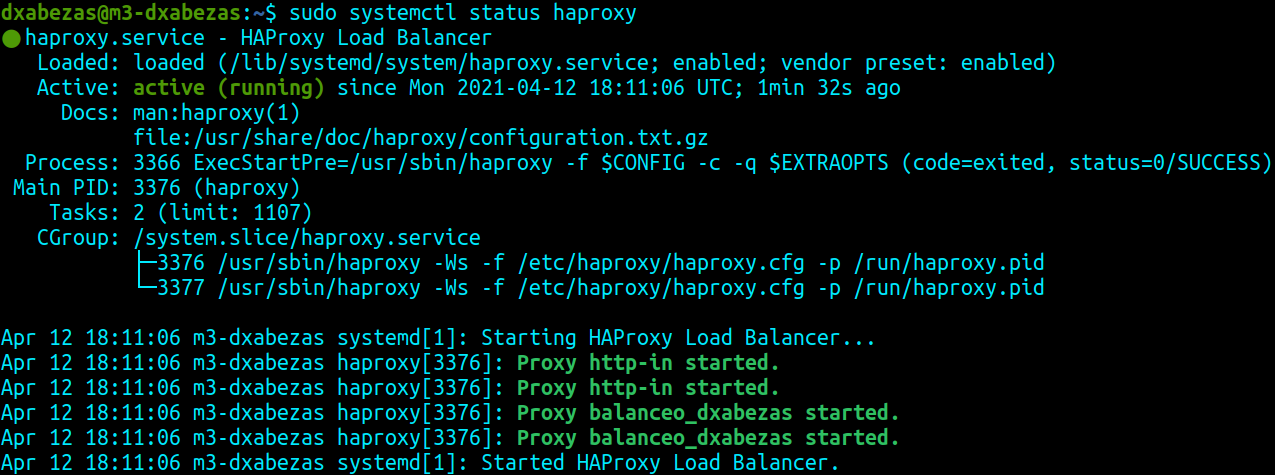
\includegraphics[width=160mm]{imgs/haproxy-status}
	\label{fig:haproxy-status}
\end{figure}

Si ahora accedemos a \texttt{192.168.56.103} desde el navegador, observamos que las dos máquinas se turnan para
servirnos su \texttt{index.html}.

Ahora configuramos la ponderación.

\begin{Verbatim}[tabsize=4]
frontend http-in
	bind *:80
	default_backend balanceo_dxabezas

backend balanceo_dxabezas
	server  m1 192.168.56.101:80 maxconn 32 weight 2
	server  m2 192.168.56.102:80 maxconn 32 weight 1
\end{Verbatim}
Si refrescamos la página nos atiende M1, M1, M2, M1, M1, M2, M1, M1, M2, \ldots

Ahora buscaremos algunas opciones avanzadas. Seleccionamos balanceo por IP-HASH. 

\begin{Verbatim}[tabsize=4]
frontend http-in
	bind *:80
	default_backend balanceo_dxabezas

backend balanceo_dxabezas
	balance source
	hash-type consistent
	server  m1 192.168.56.101:80 maxconn 32
	server  m2 192.168.56.102:80 maxconn 32
\end{Verbatim}
Ahora nos atiende siempre M1.
    
Finalmente, ponemos M1 en modo \texttt{backup}. Debemos añadir \texttt{check}, ya que no se activa el servidor de
backup si check no devuelve \texttt{DOWN}. Si no añadimos la comprobación, las peticiones no son atendidas.
\begin{Verbatim}[tabsize=4]
frontend http-in
	bind *:80
	default_backend balanceo_dxabezas

backend balanceo_dxabezas
	server  m1 192.168.56.101:80 maxconn 32 check backup
	server  m2 192.168.56.102:80 maxconn 32 check
\end{Verbatim}
Nos atiende siempre M2, pero cuando apagamos el servicio Apache2 en M2, pasa a atendernos siempre M1.

\section{Estadísticas de HAproxy}


\end{document}
